\documentclass[11pt]{article}

% ------------------------------------------------------------
% QM9 Molecular Property Prediction Project Report
% Author: Ahmadreza Rajabi
% ------------------------------------------------------------

\usepackage[margin=1in]{geometry}
\usepackage{graphicx}
\usepackage{booktabs}
\usepackage{amsmath}
\usepackage{siunitx}
\usepackage{xcolor}
\usepackage{hyperref}
\usepackage{enumitem}
\usepackage{fancyhdr}
\usepackage{titlesec}
\usepackage{listings}

\hypersetup{
    colorlinks=true,
    linkcolor=blue!60!black,
    urlcolor=blue!60!black,
    citecolor=blue!60!black
}

\pagestyle{fancy}
\fancyhf{}
\lhead{QM9 Molecular Property Prediction}
\rhead{Ahmadreza Rajabi}
\cfoot{\thepage}

\titleformat{\section}{\large\bfseries\color{blue!45!black}}{\thesection}{0.6em}{}
\titleformat{\subsection}{\normalsize\bfseries\color{blue!35!black}}{\thesubsection}{0.6em}{}

\lstset{
    basicstyle=\ttfamily\small,
    breaklines=true,
    frame=single,
    columns=fullflexible,
    backgroundcolor=\color{gray!6}
}

\title{\textbf{QM9 Molecular Property Prediction with Graph Neural Networks}}
\author{
Ahmadreza Rajabi (\texttt{arajabis})\\
Department of Chemistry\\
University of California, Irvine
}
\date{\today}

\begin{document}

\maketitle

\begin{abstract}
This project develops a graph neural network workflow for predicting quantum-chemical properties of small organic molecules from the QM9 dataset. The current implementation uses PyTorch Geometric to represent molecules as graphs, where atoms are treated as nodes and bonds/interatomic information are treated as edges. A message-passing neural network is trained to predict the HOMO--LUMO gap from molecular graph features. The immediate goal is to build a clean, reproducible demonstration of molecular machine learning for quantum-property prediction. Longer-term goals include training on larger subsets of QM9, comparing performance across dataset sizes, extending the model to additional quantum-chemical targets, and eventually testing more advanced molecular graph architectures.
\end{abstract}

\section{Project Motivation}

Accurate prediction of molecular properties is central to computational chemistry, molecular design, and materials discovery. Many important properties, such as orbital energies, atomization energies, dipole moments, and thermodynamic quantities, can be obtained from quantum-chemical calculations. However, direct quantum-chemical calculations can become expensive when many candidate molecules must be screened.

Machine learning offers a complementary strategy. Instead of performing a new quantum-chemical calculation for every molecule, a model can be trained on reference calculations and then used to rapidly estimate molecular properties for new structures. In this project, the reference data come from the QM9 dataset, which contains density-functional-theory-computed properties for approximately 134,000 small organic molecules.

The purpose of this repository is not to claim a state-of-the-art benchmark. Rather, it is designed as a clear and reproducible molecular machine-learning workflow that demonstrates how quantum-chemical data, molecular graph representations, and graph neural networks can be combined.

\section{Scientific Goal}

The primary target in the current version is the HOMO--LUMO gap. In quantum chemistry, the HOMO is the highest occupied molecular orbital and the LUMO is the lowest unoccupied molecular orbital. The HOMO--LUMO gap is a useful descriptor related to molecular electronic structure, chemical stability, and reactivity trends.

The model learns a mapping of the form
\begin{equation}
    G_{\mathrm{mol}} \longrightarrow y,
\end{equation}
where $G_{\mathrm{mol}}$ is a molecular graph and $y$ is the target quantum-chemical property. In the current run, $y$ is the HOMO--LUMO gap.

\section{Molecular Graph Representation}

In this project, each molecule is represented as a graph:
\begin{itemize}[leftmargin=1.5em]
    \item \textbf{Nodes} represent atoms.
    \item \textbf{Edges} represent bonds or pairwise molecular connectivity.
    \item \textbf{Node features} encode atom-level information.
    \item \textbf{Edge features} encode bond-level and distance-related information.
\end{itemize}

This representation is natural for chemistry because molecular properties depend strongly on how atoms are connected and how local chemical environments influence one another.

\section{Basic Idea of Graph Neural Networks}

A graph neural network updates the representation of each atom by passing information between neighboring atoms. In a message-passing model, each atom receives messages from its neighbors, combines those messages with its current representation, and updates its internal feature vector.

A simplified message-passing update can be written as
\begin{equation}
    h_i^{(k+1)} =
    \phi\left(
    h_i^{(k)},
    \sum_{j \in \mathcal{N}(i)}
    m\left(h_i^{(k)}, h_j^{(k)}, e_{ij}\right)
    \right),
\end{equation}
where $h_i^{(k)}$ is the feature vector of atom $i$ at layer $k$, $\mathcal{N}(i)$ is the set of neighboring atoms, $e_{ij}$ is the edge feature between atoms $i$ and $j$, $m$ is a message function, and $\phi$ is an update function.

After several message-passing layers, the model pools all atom representations into one graph-level molecular representation. That molecular representation is then passed through a neural network readout layer to predict the target property.

\section{What Is an Epoch?}

An epoch is one complete pass through the training dataset. For example, if the training set contains 1,600 molecules and the batch size is 64, then one epoch consists of processing the training molecules in batches until all 1,600 molecules have been used once for training.

More epochs usually give the model more chances to learn patterns in the data. However, too many epochs can lead to overfitting, where the model performs well on the training data but poorly on unseen test molecules. This is why the workflow tracks validation loss during training.

\section{Repository Structure}

The repository is organized as follows:

\begin{lstlisting}
qm9-property-prediction/
|- README.md
|- requirements.txt
|- environment.yml
|- LICENSE
|- src/
|  |- model.py
|  `- train.py
|- scripts/
|  `- run_hpc3.slurm
|- figures/
|  |- learning_curve.png
|  `- predicted_vs_actual.png
`- results/
   `- metrics.json
\end{lstlisting}

\subsection{Main Files}

\begin{itemize}[leftmargin=1.5em]
    \item \texttt{src/model.py}: defines the message-passing graph neural network.
    \item \texttt{src/train.py}: loads QM9, selects the target property, trains the model, evaluates performance, and saves results.
    \item \texttt{requirements.txt}: lists required Python packages.
    \item \texttt{environment.yml}: provides a conda-style environment specification.
    \item \texttt{scripts/run\_hpc3.slurm}: draft SLURM submission script for running larger jobs on HPC3.
\end{itemize}

\section{What the Code Does}

The training script follows these main steps:

\begin{enumerate}[leftmargin=1.5em]
    \item \textbf{Load QM9}: The dataset is downloaded and processed automatically by PyTorch Geometric.
    \item \textbf{Select target}: The current default target is target index 4, the HOMO--LUMO gap.
    \item \textbf{Construct molecular graphs}: Each molecule is represented as a graph with atom and edge features.
    \item \textbf{Split data}: The selected subset is divided into training, validation, and test sets.
    \item \textbf{Normalize targets}: The target values are normalized using the training-set mean and standard deviation.
    \item \textbf{Train the model}: The message-passing neural network is optimized using mean-squared error loss.
    \item \textbf{Track validation loss}: The best model is saved based on validation performance.
    \item \textbf{Evaluate on test set}: The final model is evaluated on unseen molecules.
    \item \textbf{Save outputs}: The code saves metrics, a learning-curve plot, and a predicted-versus-DFT plot.
\end{enumerate}

\section{Initial Smoke-Test Run}

An initial smoke test was performed to confirm that the full workflow runs correctly. This run used a small subset of the data and only two epochs. The purpose was not to obtain final performance, but to verify that dataset loading, graph construction, training, evaluation, plotting, and output saving all work.

\subsection{Command}

\begin{lstlisting}
python src/train.py --subset 2000 --epochs 2 --batch-size 64 --hidden-dim 64 --device cpu
\end{lstlisting}

\subsection{Smoke-Test Configuration}

\begin{table}[h!]
\centering
\begin{tabular}{ll}
\toprule
Setting & Value \\
\midrule
Target & HOMO--LUMO gap \\
QM9 target index & 4 \\
Subset size & 2,000 molecules \\
Training molecules & 1,600 \\
Validation molecules & 200 \\
Test molecules & 200 \\
Epochs & 2 \\
Batch size & 64 \\
Hidden dimension & 64 \\
Model parameters & 819,905 \\
Device & CPU \\
\bottomrule
\end{tabular}
\caption{Configuration for the initial smoke-test run.}
\end{table}

\subsection{Smoke-Test Results}

\begin{table}[h!]
\centering
\begin{tabular}{ll}
\toprule
Metric & Value \\
\midrule
Test MAE & 0.518 eV \\
Test $R^2$ & 0.721 \\
Best validation MSE, normalized target & 0.300 \\
\bottomrule
\end{tabular}
\caption{Initial smoke-test performance. These results are intended only as a workflow validation, not as a final benchmark.}
\end{table}

\section{Figures}

The following figure commands assume that this \LaTeX{} file is compiled from the repository root and that the figures are stored in the \texttt{figures/} directory.

\begin{figure}[h!]
\centering
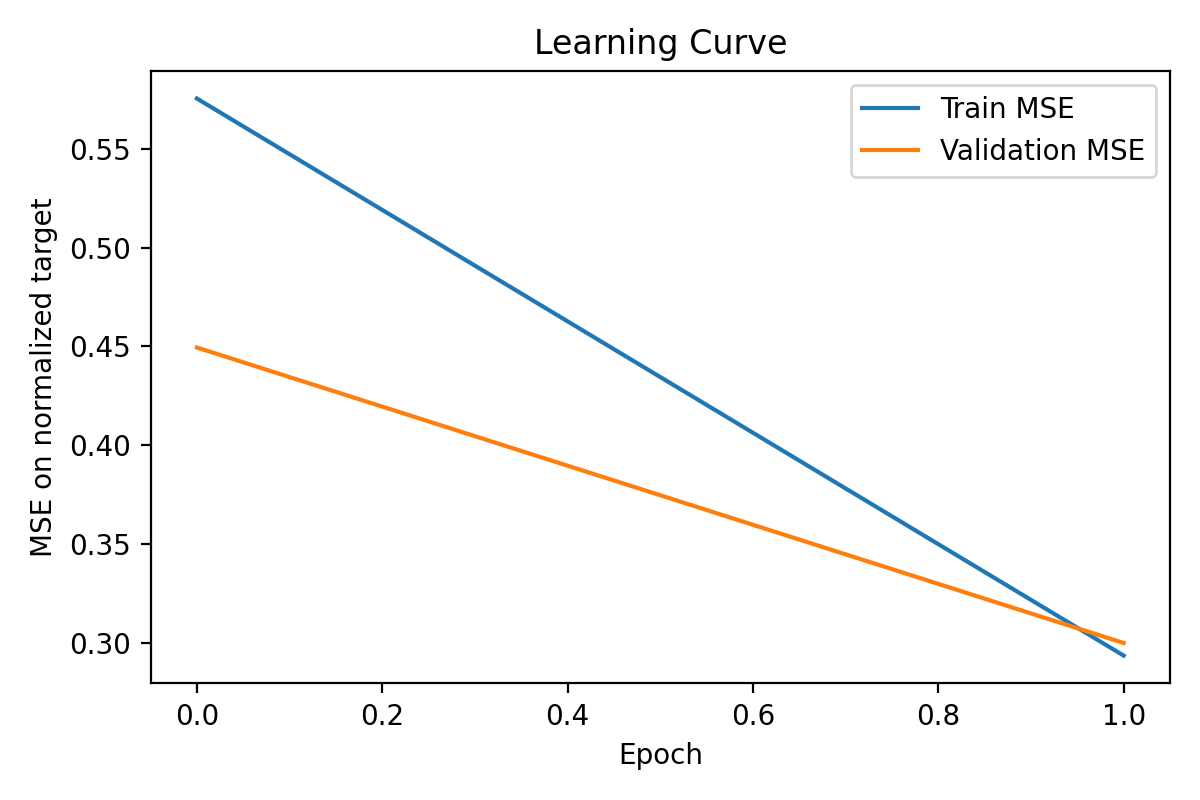
\includegraphics[width=0.72\textwidth]{figures/learning_curve.png}
\caption{Training and validation loss during the initial QM9 smoke test. The decrease in both curves indicates that the model is learning from the molecular graph data.}
\label{fig:learning_curve}
\end{figure}

\begin{figure}[h!]
\centering
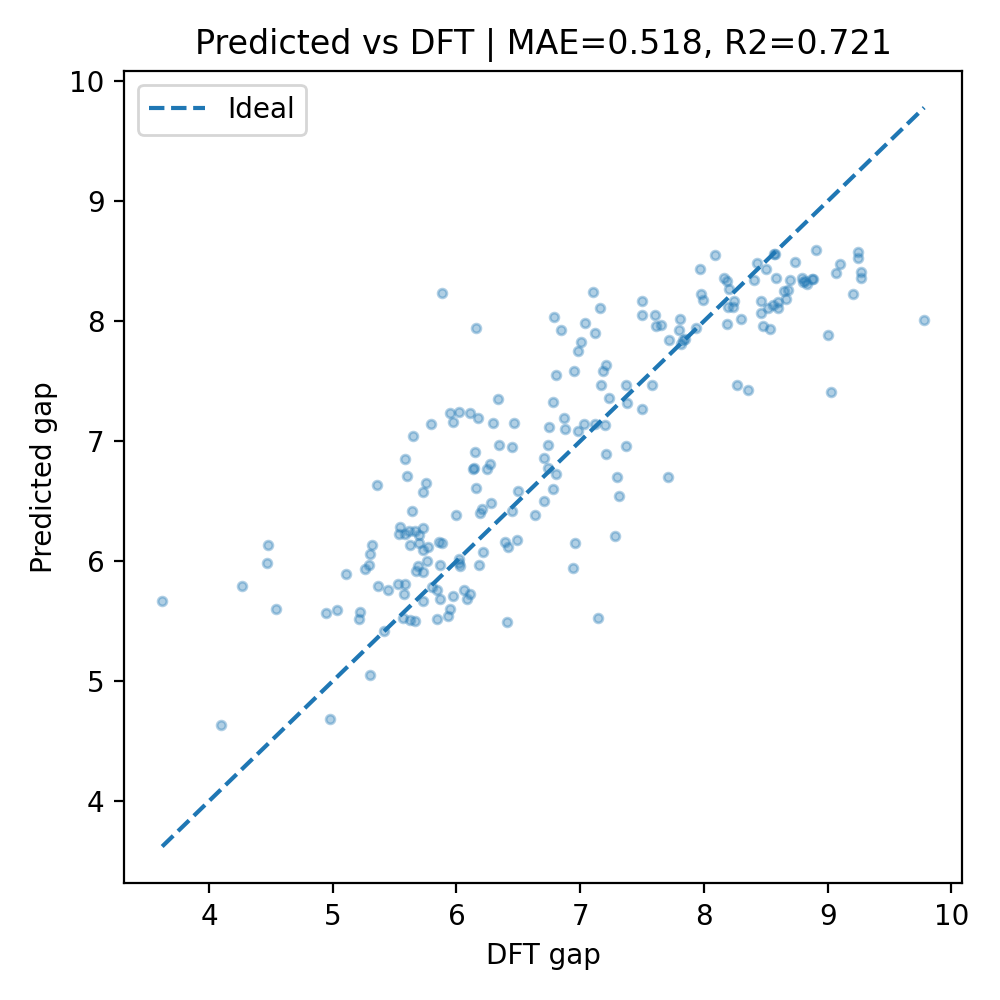
\includegraphics[width=0.65\textwidth]{figures/predicted_vs_actual.png}
\caption{Predicted HOMO--LUMO gap versus DFT reference values for the test set. The diagonal dashed line represents ideal agreement between prediction and reference.}
\label{fig:predicted_vs_actual}
\end{figure}

\section{Interpretation of the Initial Results}

The smoke-test results show that the pipeline is functioning correctly. The model completes training, validation loss decreases, and the predicted-versus-reference plot shows a clear positive correlation. Because the model was trained for only two epochs on 2,000 molecules, the results should be interpreted as a basic validation of the workflow rather than a final measure of model quality.

The current model underpredicts some high-gap molecules, which is common in early or low-data training runs. Larger training subsets, additional epochs, GPU training, and improved model architectures are expected to improve performance.

\section{Planned Next Steps}

The next stage of the project will compare model performance across dataset sizes and training settings. Planned extensions include:

\begin{enumerate}[leftmargin=1.5em]
    \item Run a larger training job using 20,000 QM9 molecules and 30 epochs.
    \item Save outputs separately under a directory such as \texttt{runs/subset\_20k\_epochs30/}.
    \item Compare the 2,000-molecule smoke test with the 20,000-molecule training run.
    \item Run full-QM9 training on HPC3 using GPU resources.
    \item Extend the workflow to additional QM9 targets, such as HOMO energy, LUMO energy, atomization energy, internal energy, and free energy.
    \item Add a comparison table summarizing MAE and $R^2$ across different training sizes.
    \item Test more advanced molecular graph models, including architectures that use 3D geometry more explicitly.
    \item Add uncertainty estimation or error analysis by molecular size and chemical composition.
\end{enumerate}

\section{Suggested Future Comparison Table}

The following table can be updated after larger calculations are complete.

\begin{table}[h!]
\centering
\begin{tabular}{lcccc}
\toprule
Run & Subset Size & Epochs & Test MAE (eV) & Test $R^2$ \\
\midrule
Smoke test & 2,000 & 2 & 0.518 & 0.721 \\
Larger subset & 20,000 & 30 & TBD & TBD \\
Full QM9 & $\sim$134,000 & 100 & TBD & TBD \\
\bottomrule
\end{tabular}
\caption{Planned comparison of model performance across training scales.}
\end{table}

\section{Summary}

This repository demonstrates a reproducible graph-neural-network workflow for quantum-chemical property prediction on QM9. The current implementation successfully loads molecular graph data, trains a message-passing neural network, evaluates HOMO--LUMO gap predictions, and generates interpretable output figures. The initial smoke test confirms that the workflow is ready for larger calculations on HPC resources.

\end{document}
